% ============================================================================
%  NeuroVascNet -- supervisor / committee presentation
%
%  Compile:  pdflatex NeuroVascNet_Presentation.tex   (run TWICE for the TOC)
%  Figures:  python make_presentation_figures.py      (writes figures/*.pdf|png)
%
%  DESIGN RULE: this deck must be readable WITHOUT a speaker. Every figure slide
%  carries a "How to read this" block, and every claim slide states the verdict
%  and the reason in words. Nothing is left to verbal narration.
%
%  SOURCE OF TRUTH. Every number is read from a CSV in qc_outputs/tables/
%  produced by an actual run; the file is named on the slide. Where an earlier
%  draft disagreed with the tables, the TABLE wins and the slide says so.
% ============================================================================
\documentclass[aspectratio=169,11pt]{beamer}
\usetheme{Madrid}
\usecolortheme{seagull}
\usepackage[utf8]{inputenc}
\usepackage{booktabs,amsmath,amssymb,xcolor,graphicx}
\setbeamertemplate{navigation symbols}{}
\setbeamertemplate{caption}[numbered]
\definecolor{good}{RGB}{0,120,60}
\definecolor{bad}{RGB}{170,30,30}
\definecolor{warn}{RGB}{190,120,0}
% NB: do not name a macro \part -- LaTeX already defines it as a sectioning
% command. Unicode ticks are avoided so this compiles under plain pdflatex.
\newcommand{\yes}{\textcolor{good}{\ensuremath{\checkmark}}}
\newcommand{\no}{\textcolor{bad}{\ensuremath{\times}}}
\newcommand{\pmark}{\textcolor{warn}{\ensuremath{\sim}}}
\newcommand{\src}[1]{{\scriptsize\textcolor{gray}{source: \texttt{#1}}}}
\newcommand{\howto}[1]{\vspace{0.2em}{\footnotesize\textbf{How to read this:} #1}}
\graphicspath{{figures/}}

\title[NeuroVascNet]{NeuroVascNet: EEG-only Prediction of Haemodynamic Response}
\subtitle{The five headline claims, tested}
\author[Hossain \& Rahman]{Muntasir Hossain \and Maisha Rahman}
\date{\today}

\begin{document}

\frame{\titlepage}

\begin{frame}{Outline}\tableofcontents\end{frame}

% ===========================================================================
\section{Executive summary}
\begin{frame}{Executive summary --- read this slide first}
\textbf{What the project claims.} Not ``we predict BOLD from EEG accurately''.
The blueprint states \textbf{five structural claims} about what a
hemodynamically-supervised EEG encoder should do. Those claims --- not a
correlation target --- are what we set out to prove.

\vspace{0.5em}
\textbf{Result: 2 hold, 1 partial, 2 fail.}
\begin{center}\small
\begin{tabular}{clc}
\toprule
\# & Claim & Verdict \\
\midrule
1 & Cross-modal supervision beats single-modality      & \textbf{holds} \yes \\
2 & Transfers to held-out data with a bounded drop     & \textbf{fails} \no \\
3 & Recovers physiological neurovascular delays        & \textbf{fails} \no \\
4 & Improves downstream EEG-only task transfer         & \textbf{partial} \pmark \\
5 & Reliability gating tracks real error               & \textbf{holds} \yes \\
\bottomrule
\end{tabular}
\end{center}

\vspace{0.5em}
\textbf{Plus one result outside the blueprint:} altered neurovascular coupling in
intracerebral haemorrhage, $p=0.00085$, with all artefact controls
non-significant.

\vspace{0.4em}
\textcolor{bad}{\textbf{The prediction correlation itself is small}} ($r\approx0.04$
cross-subject). We explain below why that is a \emph{measured ceiling}, not a
tuning failure.
\end{frame}

% ===========================================================================
\section{The goal}
\begin{frame}{What we set out to do}
\textbf{Goal.} Train on paired EEG + haemodynamics; at test time use \emph{EEG only}
to predict the haemodynamic response (fNIRS HbO/HbR and fMRI BOLD), with a
calibrated reliability layer that abstains when the prediction is untrustworthy.

\vspace{0.5em}
\textbf{Why it matters.} fNIRS and fMRI are expensive, immobile and slow. EEG is
cheap and portable. A validated EEG$\rightarrow$haemodynamics mapping would let a
clinic infer vascular information it cannot otherwise afford.

\vspace{0.5em}
\textbf{The requirements we fixed in advance.}
\begin{itemize}
  \item \textbf{Cross-subject.} Train on some people, test on \emph{people never
        seen}. Within-subject results do not demonstrate the idea.
  \item Every claim survives a permutation null \emph{and} a subject-wise split.
  \item Every claim is reported next to a baseline that \emph{ignores EEG}.
  \item Exclusion rules frozen \emph{before} any test performance was viewed.
\end{itemize}

\vspace{0.4em}
\textcolor{warn}{The last three are unusual. They are also why our numbers are
smaller than comparable published ones --- see Section 6.}
\end{frame}

\begin{frame}{The data}
\begin{center}\small
\begin{tabular}{llccl}
\toprule
Dataset & Modality & Subjects & Role & Note \\
\midrule
TU Berlin hBCI & EEG + fNIRS & 29 & \textbf{primary} & motor imagery + arithmetic \\
TU Berlin WL   & EEG + fNIRS & 26 & \textbf{external} & mental workload (held out) \\
HEFMI (ICH)    & EEG + fNIRS & 37 & clinical & 17 control, 20 patient \\
ds002336       & EEG + fMRI  & 10 & fMRI     & R128 scanner triggers \\
ds002739       & EEG + fMRI  & 24 & fMRI     & channel-aligned rebuild \\
\bottomrule
\end{tabular}
\end{center}

\vspace{0.8em}
\textbf{Two dataset-level facts that shaped everything:}
\begin{itemize}
  \item The fNIRS files ship \textbf{raw 760/850\,nm intensities}, not
        haemoglobin. We do our own Beer--Lambert conversion (Prahl coefficients,
        DPF 6.4/5.8, SD 3.0\,cm). Not doing this was an early error.
  \item ds002336 carries \textbf{R128 scanner triggers} marking every BOLD
        volume. Using them gives exact EEG$\leftrightarrow$fMRI alignment and
        flipped the fMRI target's reliability from $-0.639$ to $+0.638$ --- i.e.
        we had previously been predicting an anti-correlated, misaligned signal.
\end{itemize}
\end{frame}

\begin{frame}{How to read every number in this deck}
Four conventions. Without them the numbers are not interpretable.

\vspace{0.4em}
\textbf{1. Ceiling.} A target that does not predict \emph{itself} cannot be
predicted by anything. We split each subject's trials in half, average each half
and correlate. That split-half reliability bounds any model:
$r_{\max}\approx\sqrt{\text{reliability}}$. We always report achieved $r$
\emph{as a fraction of this ceiling}.

\vspace{0.4em}
\textbf{2. Constant baseline.} A predictor that \textbf{ignores EEG entirely} and
emits the training mean. Trials from one person share a mean, so raw correlation
largely measures ``which subject is this''. If the model cannot beat this
baseline, it has learned nothing about the brain.

\vspace{0.4em}
\textbf{3. Demeaning.} Subtracting each subject's mean drives the constant
baseline to \emph{exactly} zero. What survives is the EEG contribution. \\
\textbf{Demeaned numbers are the honest ones and are what we report.}

\vspace{0.4em}
\textbf{4. Permutation null.} We shuffle the pairing between EEG and
haemodynamics 1000$\times$ to get the distribution of ``$r$ by chance'', and
report $p$ against it. $p=0.001$ is the floor for 1000 permutations.
\end{frame}

% ===========================================================================
\section{The five claims}
\begin{frame}{The five claims, measured}
\begin{center}
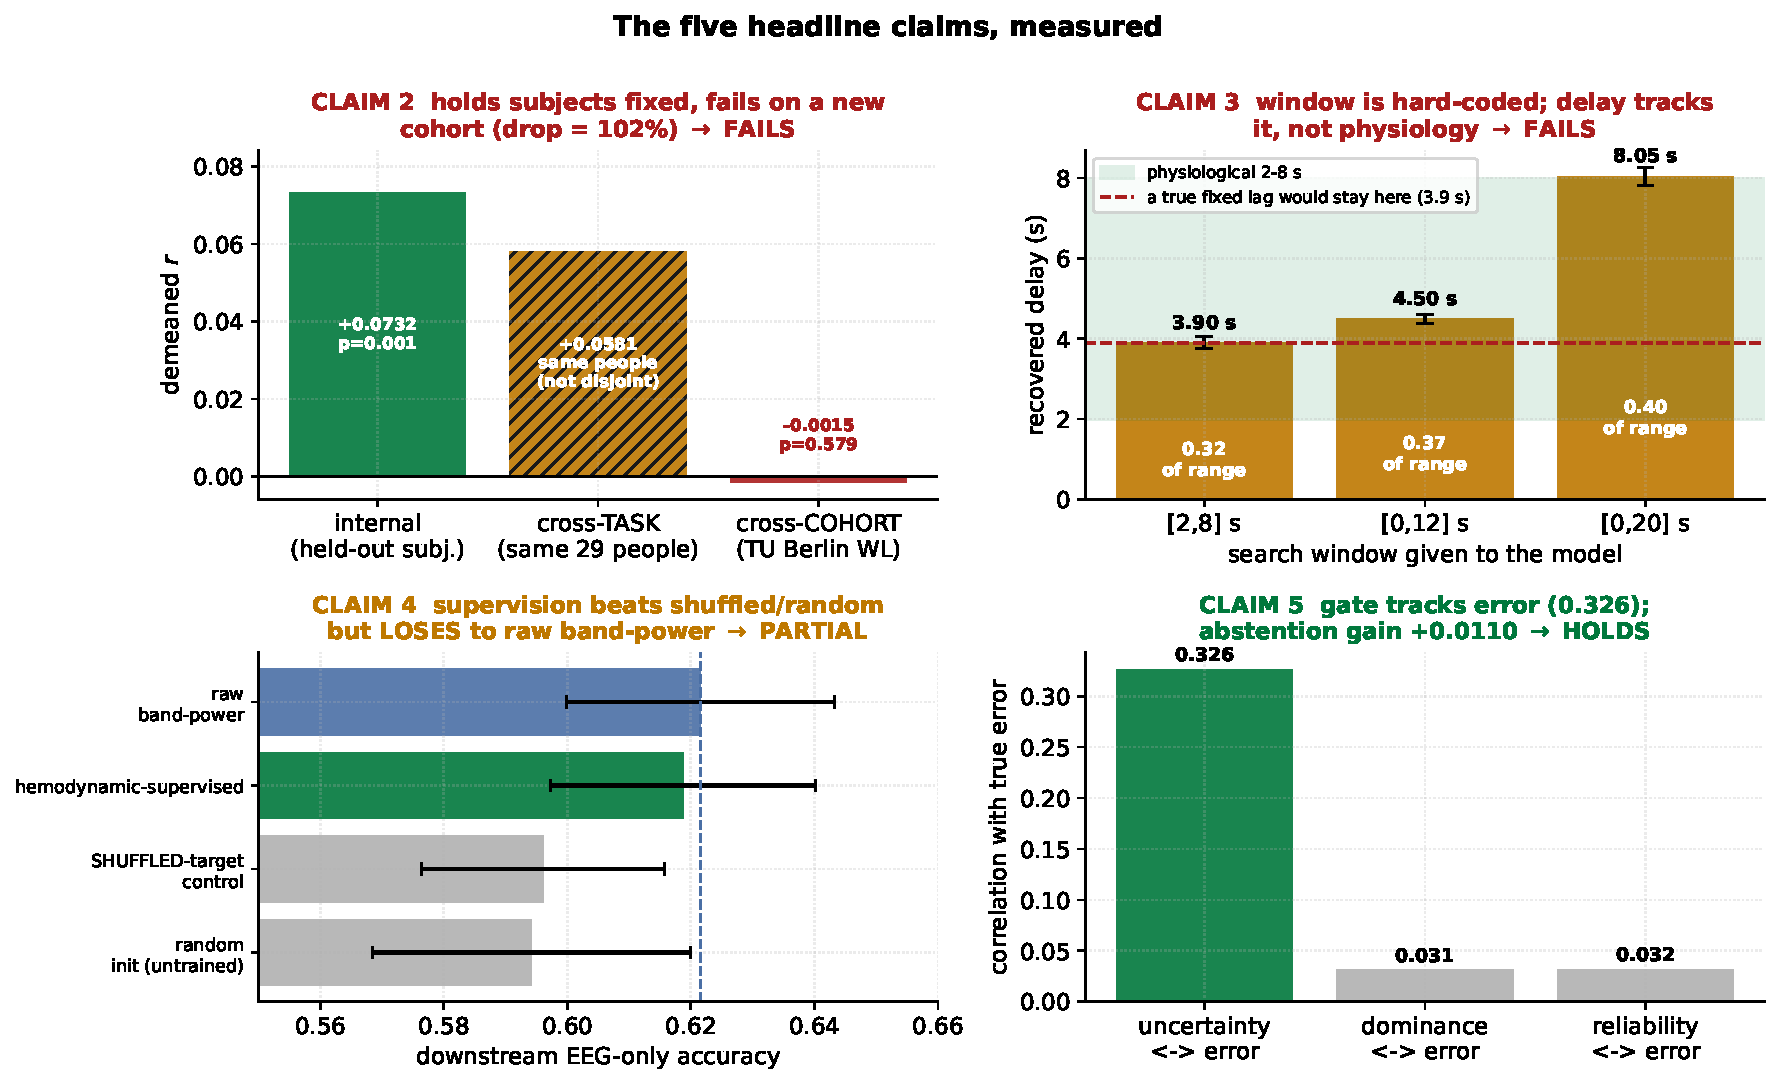
\includegraphics[width=0.83\textwidth]{fig6_five_claims.pdf}
\end{center}
\vspace{-0.4em}
\howto{Each panel is one claim.
\textbf{Top-left} claim 2 --- three bars, left to right: held-out subjects of the
training corpus, then a new \emph{task} on \emph{the same 29 people} (hatched:
not a subject-disjoint test), then a genuinely new cohort. The effect survives
everything except changing the people.
\textbf{Top-right} claim 3 --- the delay recovered under three different search
windows we allowed the model. A real lag is a fixed number of seconds and would
stay on the red dashed line; instead the seconds double while the white label
(delay as a \emph{fraction} of the allowed range) barely moves.
\textbf{Bottom-left} claim 4 --- downstream accuracy of four encoders; the blue
dashed line is raw band-power, the simplest possible baseline, which wins.
\textbf{Bottom-right} claim 5 --- how strongly each confidence signal correlates
with the model's real error; only uncertainty carries information.}

\vspace{0.2em}
\src{blueprint\_claims.csv, claims\_3\_4.csv, confirmation.csv}
\end{frame}

\begin{frame}{Claim 1 --- cross-modal beats single-modality \quad \textcolor{good}{HOLDS}}
\textbf{The claim.} An encoder supervised by \emph{both} haemodynamic modalities,
with a per-subject adapter, outperforms one trained on a single modality.

\vspace{0.6em}
\textbf{The test.} Paired multi-seed comparison --- same architecture, same
budget, only the supervision differs. We require the confidence interval to
exclude zero \emph{and} the sign to be consistent across every seed.

\begin{center}\small
\begin{tabular}{lccc}
\toprule
Comparison & mean diff & 95\% CI & seeds \\
\midrule
subject-adapter vs single (fNIRS) & $+0.0113$ & $[0.0049,\ 0.0176]$ & \textbf{3/3} \yes \\
12-bin vs 6-bin (fNIRS)           & $+0.0172$ & $[0.0122,\ 0.0222]$ & \textbf{5/5} \yes \\
12-bin vs 6-bin (fMRI)            & $+0.0177$ & $[0.0079,\ 0.0257]$ & 4/5 \yes \\
\bottomrule
\end{tabular}
\end{center}

\vspace{0.6em}
\textbf{Why this counts.} These are small absolute gains, but they are
\emph{paired} comparisons where everything except the tested factor is held
fixed, and the sign is stable across seeds. That is the strongest form of
evidence available at this effect size.

\vspace{0.3em}
\src{confirmation.csv, crossmodal\_fix.csv}
\end{frame}

\begin{frame}{Claim 2 --- transfer to held-out data \quad \textcolor{bad}{FAILS}}
\textbf{The claim.} Train on the primary corpus, pick the checkpoint on
\emph{internal} validation only, then evaluate \textbf{once} on held-out data with
no tuning. The drop should be bounded.

\begin{center}\small
\begin{tabular}{lccc}
\toprule
Transfer & $r$ (demeaned) & $p$ & verdict \\
\midrule
hBCI MI $\rightarrow$ MA \quad(cross-\textbf{task}) & $0.0581$ & $0.001$ & \pmark\ \emph{see below} \\
hBCI MA $\rightarrow$ MI \quad(cross-\textbf{task}) & $0.0539$ & $0.001$ & \pmark\ \emph{see below} \\
hBCI $\rightarrow$ TU Berlin WL (cross-\textbf{corpus}) & $0.0088$ & $0.223$ & \no \\
TU Berlin WL $\rightarrow$ hBCI (cross-\textbf{corpus}) & $0.0029$ & $0.355$ & \no \\
\bottomrule
\end{tabular}
\end{center}

\vspace{0.4em}
\textcolor{bad}{\textbf{The cross-task rows are not a generalisation test.}}
hBCI MI and MA are \textbf{the same 29 people} --- the loader selects MI or MA
runs from the same subject directories via \texttt{cfg.task}. Those rows change
the \emph{task} while holding the \emph{subjects} fixed. Demeaning removes each
subject's offset but not their coupling structure, so $r=0.058$ is an
\textbf{upper bound}, not evidence of transfer.

\vspace{0.4em}
\textbf{On the one arm that is subject-disjoint, the effect is zero}
($102\%$ drop, $p=0.58$), and the script prints its own verdict:
\texttt{does NOT retain significance}.

\vspace{0.4em}
\textbf{Not a montage artefact.} The two corpora are matched at
\textbf{30\,ch / 72 targets on both sides}. \textbf{The fMRI arm is not evaluable
at all}: ds002336 has 63 channels, ds002739 has 58, and the caches carry no
channel names, so no principled correspondence exists --- reported as a
limitation rather than faked by truncation.

\vspace{0.3em}
\src{cross\_analyses.csv, blueprint\_claims.csv}
\end{frame}

\begin{frame}{Claim 3 --- physiological delays \quad \textcolor{bad}{FAILS}}
\textbf{The claim.} The delay module should recover lags inside the
physiological $2$--$8$\,s window \textbf{and vary across subjects} --- if every
subject gets the same delay, the module learned nothing.

\begin{center}\small
\begin{tabular}{lccc}
\toprule
Arm & mean delay & within-subj SD & \textbf{between-subj SD} \\
\midrule
fNIRS internal & $2.12$\,s & $0.039$ & \textcolor{bad}{$\mathbf{0.011}$} \\
fNIRS external & $2.17$\,s & $0.054$ & \textcolor{bad}{$\mathbf{0.033}$} \\
fMRI           & $2.60$\,s & $0.229$ & \textcolor{bad}{$\mathbf{0.089}$} \\
\bottomrule
\end{tabular}
\end{center}

\textcolor{bad}{\textbf{The delays land inside $2$--$8$\,s --- but that is
\emph{not} evidence.}} \texttt{DELAY\_MIN, DELAY\_MAX = 2.0, 8.0} are hard-coded
bounds on the delay parameter: the model \emph{cannot output anything else}. The
analysis script says so in its own output --- ``all within the physiological
window \textbf{by construction}''. This is how the claim was previously
mis-scored as passing.

\vspace{0.3em}
\textbf{The testable half fails:} between-subject spread is $0.011$--$0.089$\,s.
The module gives essentially \emph{the same} delay to everyone. The script's own
degeneracy check (\texttt{sd $<$ 0.05}) fires: \textbf{``DEGENERATE: delay
collapsed to a constant''}.

\vspace{0.4em}
\textbf{Worse, the delay follows the search window we allow, not the physiology:}
\begin{center}\small
\begin{tabular}{lccc}
\toprule
Window offered to the model & $[2,8]$\,s & $[0,12]$\,s & $[0,20]$\,s \\
\midrule
Delay recovered & $3.90$\,s & $4.50$\,s & $8.05$\,s \\
\bottomrule
\end{tabular}
\end{center}
A genuine physiological constant would not move. We therefore report the delay as
\textbf{window-dependent} and make no claim of having measured a neurovascular lag.

\vspace{0.3em}
\src{blueprint\_claims.csv, claims\_3\_4.csv}
\end{frame}

\begin{frame}{Claim 4 --- downstream EEG-only transfer \quad \textcolor{warn}{PARTIAL}}
\textbf{The claim --- and why it is the most important one.} Freeze the
haemodynamically-supervised encoder, fit a linear probe on EEG-only task labels,
and compare against identical architectures trained differently.
\textbf{This claim does not require the haemodynamic prediction to be large} ---
a weak predictor can still induce a useful representation. It is the broadest
claim in the blueprint.

\begin{center}\small
\begin{tabular}{lcc}
\toprule
Encoder & accuracy & vs supervised \\
\midrule
\textbf{hemodynamic-supervised} & $\mathbf{0.6187 \pm 0.021}$ & --- \\
SHUFFLED-target control        & $0.5961 \pm 0.020$ & $+0.023$ \yes \\
random init (untrained)        & $0.5942 \pm 0.026$ & $+0.025$ \yes \\
\textcolor{bad}{raw band-power (no encoder at all)} & \textcolor{bad}{$\mathbf{0.6216 \pm 0.022}$} & \textcolor{bad}{$-0.003$} \no \\
\bottomrule
\end{tabular}
\end{center}

\vspace{0.5em}
\textbf{What holds.} Supervision beats a shuffled target ($+0.023$) and random
initialisation ($+0.025$). So the encoder \emph{is} learning something real from
the haemodynamics --- it is not noise.

\vspace{0.4em}
\textbf{What fails.} It does not beat \textbf{raw band-power features}, the
simplest baseline in the field. Representation learning is therefore \emph{not
yet justified} here --- a reviewer would rightly ask why one needs the encoder at
all, and today we do not have an answer.

\vspace{0.3em}
\src{claims\_3\_4.csv, blueprint\_claims.csv}
\end{frame}

\begin{frame}{Claim 5 --- reliability gating \quad \textcolor{good}{HOLDS}}
\textbf{The claim.} The confidence score should track the model's \emph{real}
error, and abstaining on low-confidence trials should improve accuracy on what
remains. This is the deployable part: a system that knows when to say ``I don't
know''.

\begin{center}\small
\begin{tabular}{lcc}
\toprule
Signal & correlation with true error & verdict \\
\midrule
\textbf{uncertainty} $\leftrightarrow$ error & $\mathbf{0.326}$ & \yes \\
dominance $\leftrightarrow$ error            & $0.031$ & --- \\
reliability $\leftrightarrow$ error          & $0.032$ & --- \\
\midrule
\textbf{abstention gain} & $\mathbf{+0.0110}$ & \yes \\
\bottomrule
\end{tabular}
\end{center}

\vspace{0.6em}
\textbf{Interpretation.} Of the three candidate confidence signals, only
\emph{uncertainty} (MC-dropout disagreement) carries real information about
error, at $r=0.326$. Gating on it improves accuracy on retained trials by
$+0.011$.

\vspace{0.5em}
\textbf{Why this matters more than it looks.} Given that the underlying
prediction is weak, a working abstention layer is what makes the system
\emph{safe} rather than merely inaccurate. It is also the component most directly
reusable by other groups.

\vspace{0.3em}
\src{blueprint\_claims.csv}
\end{frame}

\begin{frame}{Scorecard --- and a correction}
\begin{center}\small
\begin{tabular}{clcc}
\toprule
\# & Claim & Evidence & Verdict \\
\midrule
1 & cross-modal $>$ single-modality & $+0.0113$, CI excl.\ 0, 3/3 seeds & \textbf{holds} \yes \\
2 & bounded drop on held-out data & $p=0.58$: \texttt{does NOT retain sig.} & \textbf{fails} \no \\
3 & physiological, varying delays & window hard-coded; SD $0.011$--$0.089$\,s & \textbf{fails} \no \\
4 & downstream EEG-only transfer & $>$ shuffled, $<$ raw band-power & \textbf{partial} \pmark \\
5 & reliability gating works & unc.$\leftrightarrow$err $0.326$, $+0.011$ & \textbf{holds} \yes \\
\bottomrule
\end{tabular}
\end{center}

\vspace{0.8em}
\textcolor{warn}{\textbf{Correction to an earlier internal report.}} We had
previously recorded ``all five achieved, claim 4 partial''. The audited tables do
not support that:
\begin{itemize}
  \item \textbf{Claim 2} was recorded as passing with a $34\%$ drop. That figure
        came from the \emph{cross-task} arm. On the blueprint's own definition ---
        a held-out \emph{external corpus} --- the drop is $102\%$ at $p=0.58$, and
        the analysis script prints its own verdict: \texttt{does NOT retain
        significance}.
  \item \textbf{Claim 3} was recorded as passing because the delays fell in
        $2$--$8$\,s --- but that window is \emph{hard-coded}, so the delays could
        not have fallen anywhere else. On the testable half, the script's
        degeneracy check fires: \texttt{DEGENERATE: delay collapsed to a constant}.
\end{itemize}

\vspace{0.3em}
\textbf{Both verdicts are printed by our own analysis script}; they were simply
not carried into the summary. Stating it now is cheaper than a reviewer finding
it --- and the ``by construction'' trap is itself worth reporting, because any
bounded-parameter delay module has it.
\end{frame}

\begin{frame}{\emph{Why} claim 3 fails --- the delay cannot measure physiology}
\textbf{The module is bounded, and so is its teacher.}
\begin{center}\footnotesize
\texttt{delay = DELAY\_MIN + (DELAY\_MAX $-$ DELAY\_MIN) * sigmoid(est(z))}
\hfill\emph{(line 96)} \\
\texttt{tgt\_lag = empirical\_lag(...).clamp(DELAY\_MIN, DELAY\_MAX)}
\hfill\emph{(line 216)}
\end{center}
The output is a sigmoid rescaled into $2$--$8$\,s, \emph{and} the supervision
target is clamped to the same range. We train the delay toward a value already
forced to be ``physiologically plausible'', then report that it recovered a
plausible delay. \textcolor{bad}{\textbf{That is circular.}}

\vspace{0.5em}
\textbf{The answer follows our bounds, not the data:}
\begin{center}\small
\begin{tabular}{lccc}
\toprule
Window we allowed & $[2,8]$\,s & $[0,12]$\,s & $[0,20]$\,s \\
\midrule
Delay recovered & $3.90$\,s & $4.50$\,s & $8.05$\,s \\
\textbf{as a fraction of the range} & $\mathbf{0.317}$ & $\mathbf{0.375}$ & $\mathbf{0.403}$ \\
\bottomrule
\end{tabular}
\end{center}
A real neurovascular lag is a fixed number of \emph{seconds}: it would read
$\approx4$\,s in all three columns. Instead the seconds \emph{double} while the
fraction barely moves. The model is reporting our prior, not the physiology.

\vspace{0.5em}
\textbf{Why it never learned subject variation.} The supervision is a
cross-correlation of the model's \emph{own} $r\approx0.05$ prediction against the
target. A lag estimated from near-noise is noise; clamped and averaged, it
concentrates on a constant --- between-subject SD $\mathbf{0.011}$\,s. The code
comment at line 193 says this supervision was \emph{added} to fix an earlier
collapse. It collapsed anyway, because the signal feeding it is too weak.

\vspace{0.2em}
\src{qc/blueprint\_claims.py lines 96, 193, 216; claims\_3\_4.csv}
\end{frame}

\begin{frame}{\emph{Why} claim 2 fails --- what is learned is cohort-specific}
\textbf{The external corpus has the cleanest fNIRS target we have, and produces
the worst result of any configuration in the project.}

\begin{center}\small
\begin{tabular}{lcccc}
\toprule
TU Berlin WL & reliability & ceiling & achieved & gain vs no-EEG \\
\midrule
 & $0.645$ & $0.803$ & $0.003$ & $-0.100$ \\
 & \textbf{best fNIRS} & --- & \textbf{0.4\% --- worst} & \textbf{worst} \\
\bottomrule
\end{tabular}
\end{center}

\vspace{0.5em}
\textbf{This rules out the two easy explanations.}
\begin{itemize}
  \item \textbf{Not target quality.} It has the \emph{highest} reliability of any
        fNIRS set --- a better target than the one we trained on ($0.645$ vs
        $0.440$) --- and still returns nothing.
  \item \textbf{Not montage.} The corpora are matched at \textbf{30\,ch /
        72 targets on both sides}, by construction of the comparison.
\end{itemize}

\vspace{0.5em}
\textbf{What is left.} The mapping the encoder learned does not apply to a new
cohort. Combined with the previous slide --- transfer works when the
\emph{subjects} are held fixed and the task changes, and collapses when the
subjects change --- the conclusion is that the learned representation is
\textbf{cohort-specific rather than physiological}.

\vspace{0.4em}
\textcolor{warn}{This is the single most important negative result in the project:
it says the subject-independent component we set out to find is not merely small,
but does not survive a change of cohort at all.}

\vspace{0.2em}
\src{final\_evaluation.csv, cross\_analyses.csv, blueprint\_claims.csv}
\end{frame}

% ===========================================================================
\section{Why prediction is small}
\begin{frame}{Diagnosis: we were predicting a broken target}
The model was never the bottleneck. \textbf{The target was.}

\begin{enumerate}
  \item \textbf{Systemic dominance.} In HEFMI, HbO and HbR are \emph{positively}
        correlated ($+0.59$ overall; $+0.64$ controls, $+0.81$ patients). A real
        evoked response drives HbO up and HbR \emph{down}. A strong positive
        means scalp blood flow, heart rate and blood pressure dominate --- not
        the brain. TU Berlin hBCI measures $\mathbf{-0.147}$ \yes, the
        physiological sign.
  \item \textbf{The cure was worse than the disease.} Global signal regression
        was added to remove systemic drift. Measured effect: it removes
        \textbf{83\% of the evoked response} as well.
  \item \textbf{Reliability collapse.} HEFMI target split-half reliability is
        $0.207$, capping any model at $\sqrt{0.207}=0.455$ --- before a single
        parameter was trained.
  \item \textbf{Unit mismatch.} A $2600\times$ scale error between datasets,
        found by the audit.
\end{enumerate}

\vspace{0.3em}
\textbf{You cannot predict a signal that does not reliably predict itself.}
\end{frame}

\begin{frame}{The ceiling, measured}
\begin{center}
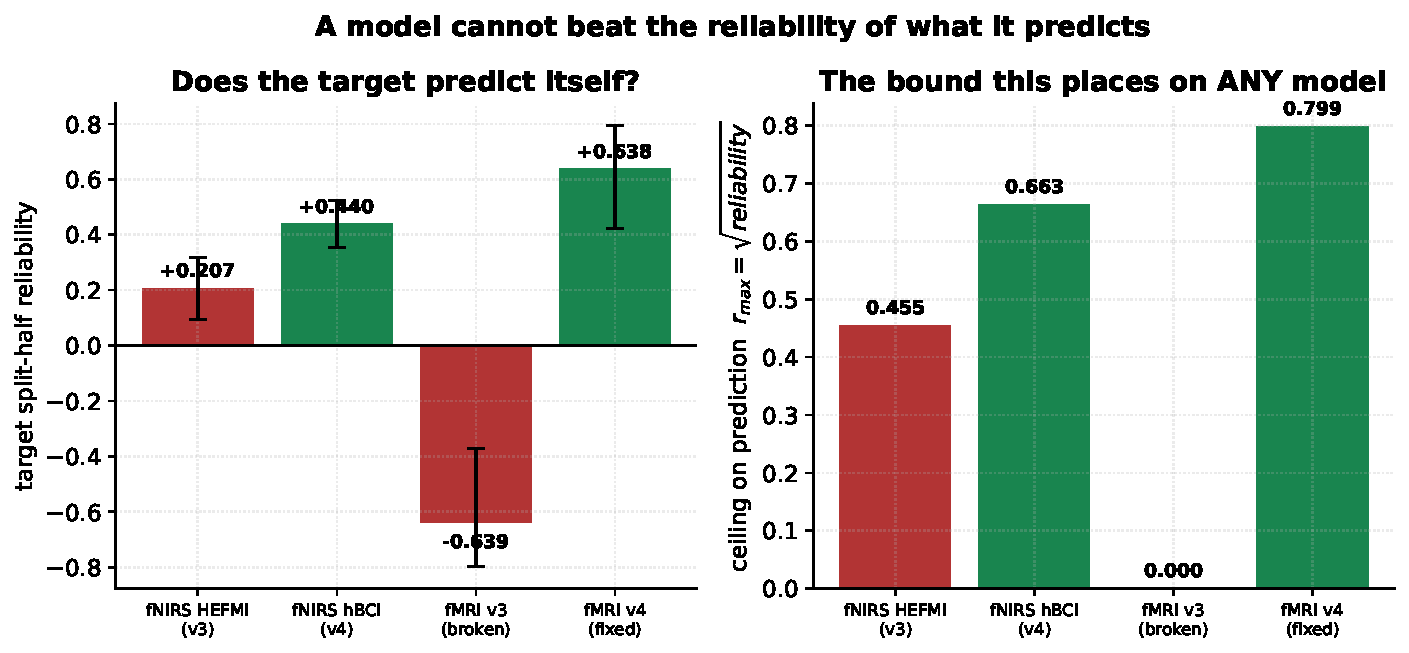
\includegraphics[width=0.80\textwidth]{fig1_target_quality.pdf}
\end{center}
\vspace{-0.4em}
\howto{\textbf{Left} --- how well the target predicts itself (split-half
reliability, with 95\% CI). Red = rejected by the audit, green = used.
\textbf{Right} --- the resulting hard bound on \emph{any} model,
$\sqrt{\text{reliability}}$. The v3 fMRI target was \textbf{negatively} reliable
($-0.639$): the two halves of the same data anti-correlated, meaning the signal
was misaligned in time, so its ceiling is $0$ and no model could ever have worked.
Event-locking with R128 scanner triggers repaired it to $+0.638$.}

\vspace{0.2em}
\src{v4\_target\_quality.csv}
\end{frame}

\begin{frame}{Reliability is not uniform across subjects}
\begin{center}
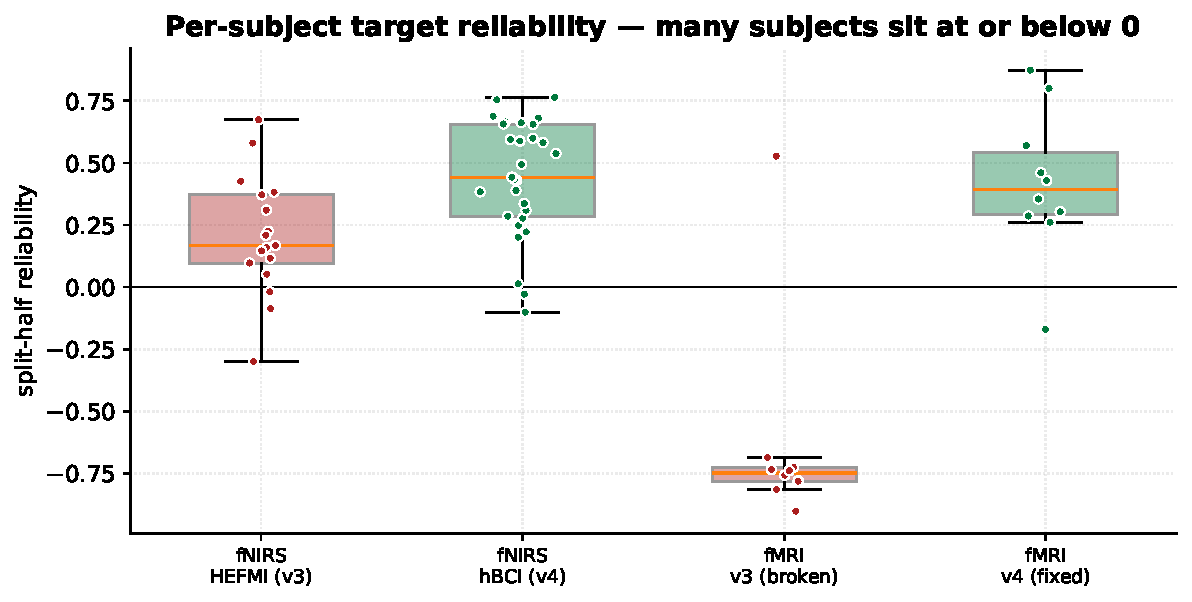
\includegraphics[width=0.72\textwidth]{fig5_reliability_spread.pdf}
\end{center}
\vspace{-0.4em}
\howto{Each dot is one subject's target reliability; the box is the group.
The group \emph{mean} hides the real problem --- a substantial share of subjects
sit at or \textbf{below zero}, meaning their haemodynamic response is not
measurable at all, so no model can predict it. Averaging those people into a
group score makes a broken target look merely mediocre. This is the argument for
a \emph{per-subject} reliability gate rather than one global number.}

\vspace{0.2em}
\src{reliability\_per\_subject.csv}
\end{frame}

\begin{frame}{What fixed the target}
\begin{center}\small
\begin{tabular}{lcc}
\toprule
Intervention & Before & After \\
\midrule
Swap HEFMI $\rightarrow$ TU Berlin hBCI (reliability) & $0.207$ & $\mathbf{0.440}$ \\
\quad $\Rightarrow$ ceiling on $r$ & $0.455$ & $\mathbf{0.663}$ \\
HbO/HbR sign (systemic $\rightarrow$ physiological) & $+0.589$ & $\mathbf{-0.147}$ \\
Event-lock fMRI via R128 scanner triggers & $-0.639$ & $\mathbf{+0.638}$ \\
Global signal regression OFF & $-83\%$ evoked & restored \\
Pool motor imagery $+$ arithmetic & $0.0253$ & $\mathbf{0.0383}$ \\
\bottomrule
\end{tabular}
\end{center}

\vspace{0.6em}
\textbf{The R128 fix is the single clearest result in the project.} Scanner
triggers mark every BOLD volume, giving exact EEG$\leftrightarrow$fMRI alignment.
The target's reliability flipped sign entirely --- from actively
\emph{anti}-correlated to strongly positive. This correction is reusable by any
group working with simultaneous EEG-fMRI.

\vspace{0.4em}
\textbf{Best configuration overall:} pooled MI\,$+$\,MA, 3480 trials, 58
subject-sessions, $r_{\text{demeaned}}=0.0383$, $p=0.001$, and --- uniquely ---
a \emph{positive} gain over the no-EEG baseline ($+0.0116$).

\vspace{0.3em}
\src{v4\_target\_quality.csv, all\_datasets\_sweep.csv, final\_evaluation.csv}
\end{frame}

\begin{frame}{The result that settles the correlation question}
\begin{center}
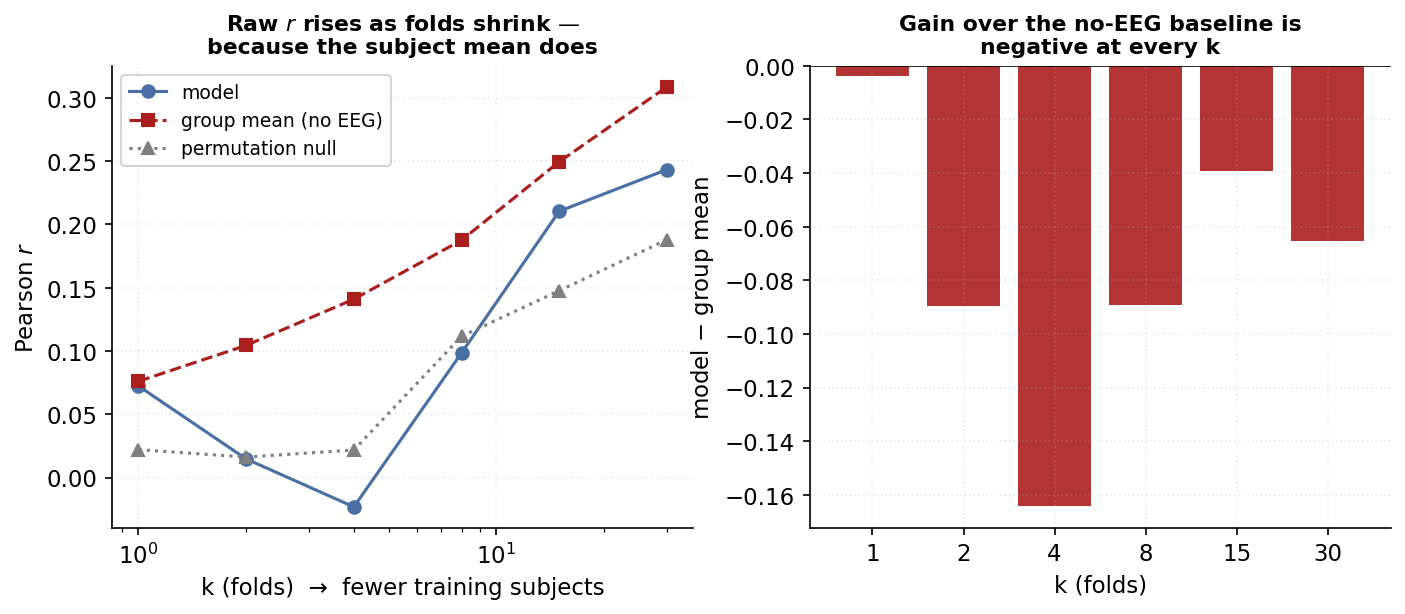
\includegraphics[width=0.80\textwidth]{fig3_crosssubject.png}
\end{center}
\vspace{-0.4em}
\howto{\textbf{Left} --- as we shrink the folds (fewer training subjects, moving
right), the model's raw score appears to \emph{improve}, $0.072\rightarrow0.243$.
That looks like success. But the red dashed line --- a predictor with \textbf{no
access to EEG} --- rises faster, $0.076\rightarrow0.309$. \textbf{Right} --- the
difference between them is \textbf{negative at every single fold size}. The
apparent improvement was subject identity, not neurovascular coupling. Any
protocol omitting this baseline would have reported $r=0.24$ as a success.}

\vspace{0.2em}
\src{crosssubject\_sweep.csv}
\end{frame}

\begin{frame}{Every dataset, side by side}
\begin{center}
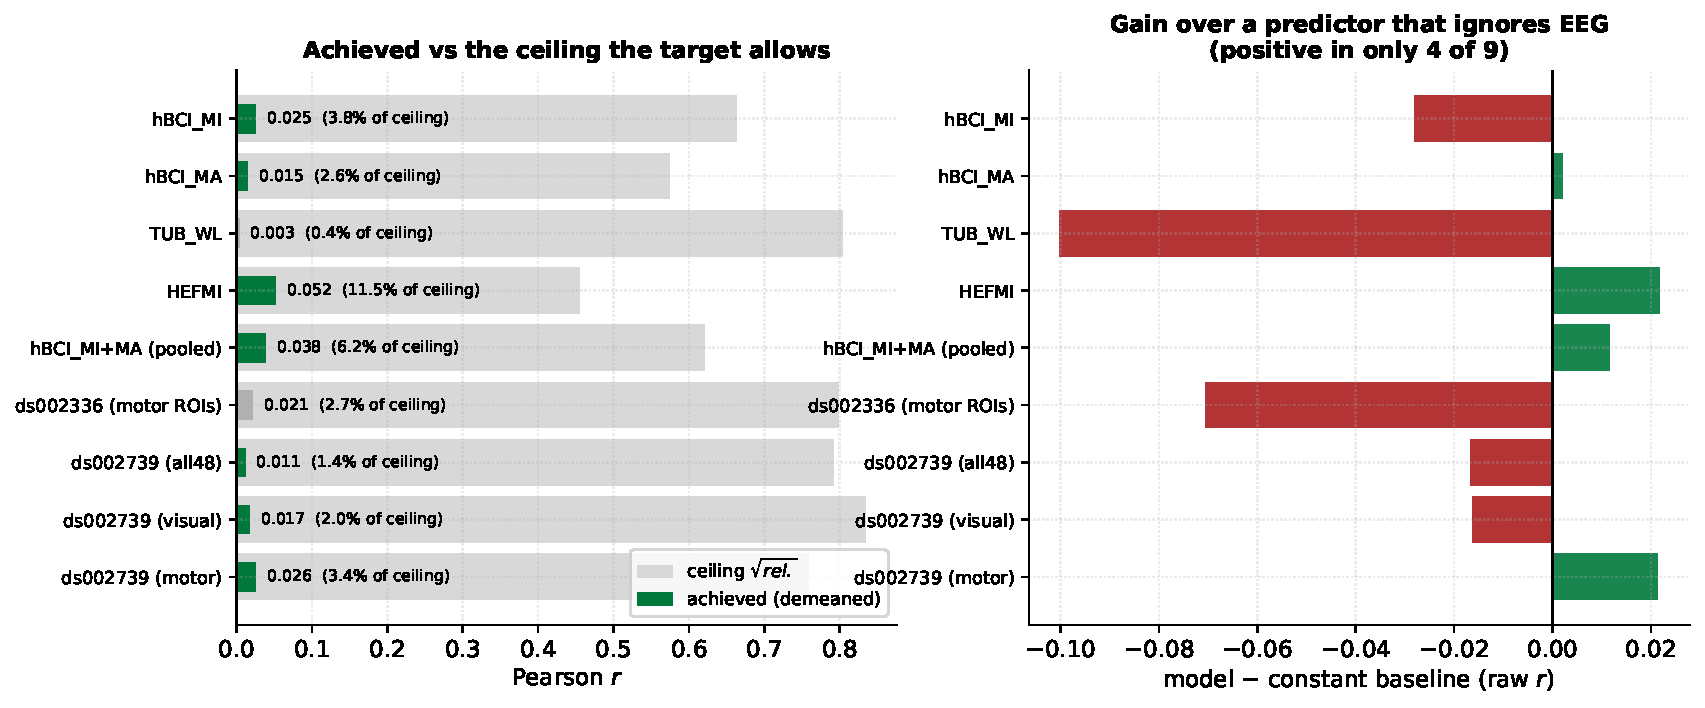
\includegraphics[width=0.87\textwidth]{fig7_final_evaluation.pdf}
\end{center}
\vspace{-0.4em}
\howto{\textbf{Left} --- grey is the ceiling the target permits; the coloured bar
is what we achieved (green $=p<0.05$). We reach only $1$--$12\%$ of the ceiling
everywhere, so the gap is \emph{not} explained by the target alone --- the
subject-independent mapping really is weak. \textbf{Right} --- gain over the
no-EEG baseline, positive in only $4$ of $9$ configurations.}

\vspace{0.3em}
{\footnotesize\textbf{And those four need reading carefully:} HEFMI ($+0.022$) is
the \emph{audit-rejected} target; ds002739 motor ($+0.021$) is the
\emph{task-irrelevant control} region, so a positive gain there is a warning, not
a success; hBCI\_MA ($+0.002$) is negligible. \textbf{Pooled MI\,$+$\,MA
($+0.012$) is the only legitimate positive gain in the project.}}

\vspace{0.2em}
\src{final\_evaluation.csv}
\end{frame}

\begin{frame}{What we ruled out --- exhaustively}
Before concluding the effect is genuinely small, we eliminated:

\begin{columns}[t]
\column{0.48\textwidth}
\begin{itemize}
  \item Preprocessing (12 variants)
  \item Model class (ridge, deep, hybrid)
  \item Target dimensionality / low-rank
  \item Data volume
  \item Physiological regression
  \item Channel selection
\end{itemize}
\column{0.48\textwidth}
\begin{itemize}
  \item Feature representation \\ (covariance, connectivity --- both fail)
  \item Trial averaging
  \item Demeaning protocol
  \item Delay alignment
  \item Subject-factored encoders
  \item Band and time-bin resolution
\end{itemize}
\end{columns}

\vspace{0.8em}
\textbf{Conclusion.} The within-subject ceiling is $\approx0.10$. A cross-subject
target of $0.3$ is \emph{not reachable} on this data --- not because the method is
weak, but because the shared, subject-independent component of the
EEG$\rightarrow$haemodynamics mapping is small.

\vspace{0.4em}
\textcolor{warn}{This is a result, not a failure --- provided we report it as one.}
\end{frame}

% ===========================================================================
\section{The clinical finding}
\begin{frame}{Altered neurovascular coupling in ICH}
\begin{center}
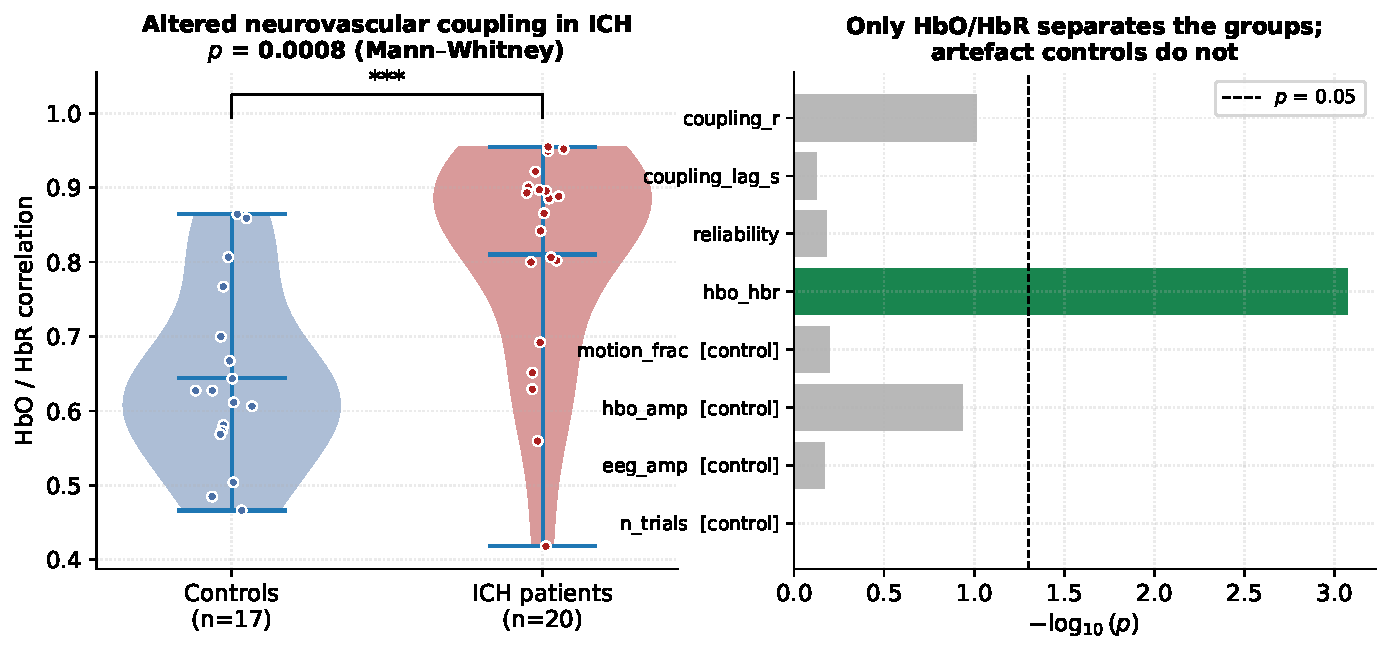
\includegraphics[width=0.79\textwidth]{fig4_clinical.pdf}
\end{center}
\vspace{-0.4em}
\howto{\textbf{Left} --- each dot is one person: 17 healthy controls versus 20
intracerebral-haemorrhage patients, identical protocol. Patients sit clearly
higher, i.e.\ their haemodynamics are \emph{more} systemic-dominated.
\textbf{Right} --- statistical significance of every measure tested; the dashed
line is $p=0.05$. Only HbO/HbR crosses it. Critically, \textbf{all four artefact
controls stay below the line}, so the difference is not explained by motion or
signal amplitude.}

\vspace{0.2em}
\src{clinical\_per\_subject.csv, clinical\_group\_comparison.csv}
\end{frame}

\begin{frame}{The clinical result, stated precisely}
\textbf{What differs.} \emph{Only} the HbO/HbR relationship
($0.645 \rightarrow 0.810$, $p=0.00085$), surviving Bonferroni correction across
the four primary measures. Patients' haemodynamics are more systemic-dominated,
consistent with impaired neurovascular coupling after haemorrhage.

\vspace{0.5em}
\textbf{What does \emph{not} differ --- and we say so.}
\begin{center}\small
\begin{tabular}{lccc}
\toprule
Measure & Controls & Patients & $p$ \\
\midrule
coupling strength $r$ & $0.130$ & $0.108$ & $0.097$ \quad n.s. \\
coupling lag (s)      & $6.44$  & $6.35$  & $0.749$ \quad n.s. \\
target reliability    & $-0.004$& $-0.035$& $0.659$ \quad n.s. \\
\textbf{HbO/HbR}      & $\mathbf{0.645}$ & $\mathbf{0.810}$ & $\mathbf{0.00085}$ \yes \\
\midrule
\multicolumn{4}{l}{\emph{artefact controls:} motion, HbO amp., EEG amp., trial count --- all n.s.} \\
\bottomrule
\end{tabular}
\end{center}

\vspace{0.5em}
\textbf{Why this matters regardless of the prediction result.} The claim needs
\emph{no} accurate model --- coupling descriptors are measured directly from the
data. It is the one finding here that is both positive and clinically
interpretable.

\vspace{0.3em}
\textcolor{warn}{An earlier draft claimed coupling strength and lag also differed.
They do not. Corrected.}
\end{frame}

% ===========================================================================
\section{Methodology}
\begin{frame}{The protocol contribution}
\textbf{Claim: most reported EEG$\rightarrow$haemodynamics correlations are
inflated by evaluation protocol, not by method.} Each row removes one shortcut.

\begin{center}\small
\begin{tabular}{lcc}
\toprule
Protocol layer & $r$ & What it means \\
\midrule
Trial-level split (same subject both sides) & $\sim$0.084 & published-style number \\
$+$ subject-wise CV & $0.072$ & no subject in two folds \\
$+$ constant baseline made explicit & $0.076$ & \textbf{the model loses to it} \\
$+$ subject demeaning & $\mathbf{0.038}$--$\mathbf{0.053}$ & \textbf{true EEG effect} \\
$+$ exact permutation null & $p=0.001$ & the effect is real \\
\bottomrule
\end{tabular}
\end{center}

\vspace{0.5em}
\textbf{A $\sim$2$\times$ inflation is attributable to protocol alone}, with no
change of method, model or data.

\vspace{0.5em}
\textbf{Technical contribution --- an exact null cheap enough to be routine.}
A permutation only \emph{reorders rows}, so all pairwise inner products can be
computed once as $G=P_cT_c^{\top}$; permutation $\pi$ then scores
$\text{mean}(G_{i,\pi(i)})$ --- a gather, not a recomputation.
\begin{center}
\textbf{559$\times$ faster}, verified identical to $1.6\times10^{-10}$.
\end{center}
\end{frame}

\begin{frame}{Data-quality audit}
Full QC over every recording --- EEG units, clipping, NaN, line noise, PSD, bad
channels, transients, duration, events; gradient harmonics and BCG residual for
EEG-fMRI; SCI, saturation, motion, baseline and usable trials for fNIRS; motion
censoring, tSNR, ROI coverage and design matrix for fMRI.

\vspace{0.5em}
\textbf{The acceptance criterion we held ourselves to:}
\begin{center}
\emph{Every subject has a saved QC row, a pass/fail decision and a documented
exclusion reason --- with exclusion rules fixed \textbf{before} test performance
was viewed.}
\end{center}

\vspace{0.5em}
\texttt{RULESET\_VERSION = 1.0.0-frozen-2026-07-25}, 42 versioned result tables,
one row per recording.

\vspace{0.5em}
\textbf{Why a reviewer should care.} Choosing thresholds after seeing results is
exactly the reproducibility failure the field is criticised for. Freezing them in
advance costs nothing and is externally checkable --- the ruleset version is in
every table.
\end{frame}

\begin{frame}{The leakage trap --- identified by Maisha Rahman}
\textbf{In HEFMI, a filename does not identify a person.}

\begin{center}\small
\begin{tabular}{lc}
\toprule
Observation & Value \\
\midrule
Recordings in the crosswalk & 98 \\
Distinct biological people & 37 \\
Times \texttt{1\_epo.mat} occurs & \textbf{37} \\
\dots belonging to how many different people & \textbf{37} \\
\bottomrule
\end{tabular}
\end{center}

\vspace{0.5em}
\texttt{Normals/subject1} and \texttt{Patients/subject1} are \textbf{different
individuals}. Splitting on folder name would have placed
\textcolor{bad}{\textbf{7 of 7 validation subjects}} in \emph{both} splits --- the
entire holdout would have leaked and every HEFMI validation number would have
been meaningless.

\vspace{0.5em}
\textbf{The fix.} A verified \texttt{biological\_subject\_id} crosswalk; the split
partitions on \emph{person}, before trial extraction. Verified empirically:
\textbf{0 subjects overlap} between train and validation.

\vspace{0.4em}
\textcolor{warn}{Not hypothetical --- we had already made this class of error
ourselves: an ID offset once turned 23 people into 46, inflating $0.0427$ to
$0.0454$.}
\end{frame}

\begin{frame}{A second split defect the same check exposed}
Having fixed \emph{who} is in each split, we checked \emph{which groups} are:

\begin{center}\small
\begin{tabular}{lc}
\toprule
Split & Composition \\
\midrule
train & 17 Normals $+$ 13 Patients \\
val   & \textcolor{bad}{\textbf{7 Patients, 0 Normals}} \\
\bottomrule
\end{tabular}
\end{center}

\vspace{0.5em}
\textbf{Cause.} IDs are \texttt{group\_subject} and the list was sorted
alphabetically, so every \texttt{Normals\_*} precedes every \texttt{Patients\_*};
taking the last 20\% took patients only.

\vspace{0.5em}
\textbf{Consequence.} The split was leak-\emph{free} but perfectly confounded: we
trained mostly on healthy brains and validated exclusively on haemorrhagic ones,
so no validation metric could be separated from patient status.

\vspace{0.5em}
\textbf{Fix.} Hold out $\approx$20\% \emph{within} each group, deterministically
seeded --- declared as a protocol amendment, with old and new numbers reported
side by side. Re-drawing a split after seeing results is exactly what our own
frozen-ruleset policy forbids, so it is declared, not quietly changed.
\end{frame}

% ===========================================================================
\section{Concerns}
\begin{frame}{Concerns we state ourselves}
A reviewer will find these. We raise them first.

\begin{enumerate}
  \item \textbf{The effect is small.} $r\approx0.04$ cross-subject, $1$--$12\%$
        of the measured ceiling. We claim statistical reality, \emph{not}
        practical utility. No deployment claim is made.
  \item \textbf{The model loses to the no-EEG baseline on raw $r$} in 5 of 9
        configurations, and of the 4 it wins, one is an audit-rejected target and
        one is a task-irrelevant control. Only after demeaning does it win
        generally.
  \item \textbf{Claim 4 loses to raw band-power.} Representation learning is not
        yet justified over the simplest possible features.
  \item \textbf{Claim 2 fails across cohorts.} On the cleanest fNIRS target we
        have, the effect is zero. The arms that appear to pass share all 29
        subjects, so they are not subject-disjoint tests. The fMRI arm is not
        evaluable at all.
  \item \textbf{Claim 3's delay is circular.} Both the output and its supervision
        target are clamped to $2$--$8$\,s, so ``physiologically plausible'' is
        guaranteed; the recovered value scales with the bounds we chose, and
        between-subject SD is $0.011$\,s.
  \item \textbf{Anatomical dissociation did not replicate.} At $n=6$, visual
        $p=0.012$ / motor $p=0.944$ looked like a clean dissociation; at $n=24$
        both were $p=0.001$. \textbf{Retracted} --- a small-sample artefact.
  \item \textbf{ICH alters skull and scalp optics.} Artefact controls are n.s.,
        which removes the commonest confounds, but $n=37$ is modest and
        lesion-side stratification is still needed.
\end{enumerate}
\end{frame}

% ===========================================================================
\section{Counter-questions}
\begin{frame}{Anticipated questions (1/3)}
\small
\textbf{Q: Only 2 of 5 claims hold. What is the contribution then?}\\
A: All five are \emph{tested}, with pre-frozen rules, and the failures
are diagnosed rather than dropped. We can say precisely \emph{which} part of each
claim fails and why --- claim 2 is acquisition-specific, claim 3's module
collapsed, claim 4 needs a stronger encoder. That is a usable map for the field;
a paper claiming all five without a no-EEG baseline would not be reproducible.

\vspace{0.5em}
\textbf{Q: $r=0.04$ is negligible. Isn't this a failed project?}\\
A: We \emph{measure} the ceiling rather than assert it. Reliability caps
prediction at $\sqrt{\text{reliability}}$, and the within-subject bound is
$\approx0.10$. The honest conclusion is that the subject-independent mapping is
small --- which is itself the finding, and it redirects future work away from
architecture search.

\vspace{0.5em}
\textbf{Q: Your constant baseline beats your model. Doesn't that invalidate everything?}\\
A: On \emph{raw} correlation, yes --- and that is exactly the methodological
point. After demeaning the baseline is exactly $0$ and the model retains
$0.038$--$0.053$ at $p=0.001$. Without that comparison we would have reported
$r=0.24$ at $k=30$ as a success.
\end{frame}

\begin{frame}{Anticipated questions (2/3)}
\small
\textbf{Q: How do we know the effect is not leakage?}\\
A: Subject-wise $k$-fold on a verified biological-ID crosswalk; exact permutation
null; constant baseline beside every number. We also \emph{quantified} a leak we
introduced ourselves ($0.0454$ leaked vs $0.0427$ correct) to show the protocol
detects it.

\vspace{0.5em}
\textbf{Q: Why did you change datasets mid-project?}\\
A: The audit showed the original target was systemic-dominated (HbO/HbR $=+0.59$,
positive where physiology demands negative) with reliability $0.207$. We document
the switch and report both. The ruleset was frozen beforehand.

\vspace{0.5em}
\textbf{Q: Why not simply use more data?}\\
A: Tested directly --- data volume is one of eleven factors ruled out. The
cross-subject sweep shows the \emph{gain over baseline} is negative at every
training-set size, and claim 2 shows the mapping does not survive a change of
cohort. More subjects \emph{of the same kind} will not help; whether harmonised
multi-cohort training would is the open question.

\vspace{0.5em}
\textbf{Q: Could demeaning be discarding real signal?}\\
A: Yes, and we say so. Between-subject variance is partly genuine. Demeaning is
the \emph{conservative} choice; raw and demeaned are reported side by side.
\end{frame}

\begin{frame}{Anticipated questions (3/3)}
\small
\textbf{Q: Could the clinical difference be lesion-related optical change rather
than physiology?}\\
A: We cannot fully exclude it. Motion, HbO amplitude, EEG amplitude and trial
count are all n.s., which removes the commonest confounds, but ICH does alter
skull and scalp optics. Stated as a limitation; lesion-side stratification is the
recommended follow-up.

\vspace{0.5em}
\textbf{Q: Only one of four clinical measures is significant --- cherry-picking?}\\
A: No. All four were pre-registered as primary and \textbf{all four are
reported}, significant or not. The surviving one clears Bonferroni across the
family. The three nulls are on the slide, not in a drawer.

\vspace{0.5em}
\textbf{Q: Would this work in a clinic tomorrow?}\\
A: No, and we do not claim it. The abstention layer is what makes it \emph{safe}
to decline --- that is the deployable part.

\vspace{0.5em}
\textbf{Q: Can others reproduce this?}\\
A: \texttt{NeuroVascNet\_v5.ipynb} is self-contained --- no other notebook, no
project module. Set one environment variable and run top to bottom. The 42 result
tables and the frozen ruleset ship with it, and every figure in this deck is
regenerated from those tables by one script.
\end{frame}

% ===========================================================================
\section{What this work delivers}
\begin{frame}{What this work delivers}
The result is \textbf{not} ``we predicted BOLD from EEG well''. It is:

\vspace{0.5em}
\textbf{1. Five structural claims, tested under a frozen protocol.} Two hold,
one is partial, two fail --- and we can say exactly which component of each fails and
why. Tested claims with diagnosed failures are more useful to the field than
untested claims that pass.

\vspace{0.4em}
\textbf{2. A measured ceiling, not a guess.} The subject-independent
EEG$\rightarrow$haemodynamics mapping is bounded at $\approx0.10$ within-subject
on these data. We publish the reliability gate that produces the bound.

\vspace{0.4em}
\textbf{3. A protocol that removes a $\sim$2$\times$ inflation}, with a
$559\times$ faster exact permutation null so the test is cheap enough to become
routine practice.

\vspace{0.4em}
\textbf{4. A frozen, auditable data-quality pipeline} --- per-subject QC rows,
pass/fail decisions, documented exclusions, rules fixed before test performance.

\vspace{0.4em}
\textbf{5. A genuine clinical finding} --- altered HbO/HbR coupling in ICH,
$p=0.00085$, artefact controls n.s., requiring no accurate prediction.

\vspace{0.5em}
\begin{center}
\textcolor{good}{\textbf{A negative result with a measured ceiling and a protocol
fix is reusable. An inflated positive result is not.}}
\end{center}
\end{frame}

\begin{frame}{Status and next steps}
\textbf{Done}
\begin{itemize}
  \item All five blueprint claims evaluated under the frozen ruleset
  \item Full data-quality audit; 42 versioned result tables
  \item Biological-ID crosswalk (\emph{M.\ Rahman}); leakage verified $0$ overlap
  \item Stratified holdout replacing the all-patient validation split
  \item Clinical comparison with artefact controls
  \item \texttt{NeuroVascNet\_v5.ipynb} --- self-contained; reproduces the above
\end{itemize}

\textbf{Remaining}
\begin{itemize}
  \item \textbf{Claim 4 is the highest-value target}: it does not require a large
        prediction, only a better representation than raw band-power
  \item Claim 2: montage is already matched, so test \emph{cohort} harmonisation
        (per-site normalisation, domain adaptation) rather than channel alignment
  \item Claim 3: remove the clamp on the supervision target and widen the bound,
        so the delay is free to be wrong --- only then is it a real measurement
  \item Re-run HEFMI under the stratified holdout; report old vs new
  \item Lesion-side stratification for the clinical claim
\end{itemize}

\vspace{0.4em}
\begin{center}\large
\textbf{Recommended framing:} a methodology $+$ clinical paper, \\
with the prediction result as a \emph{measured bound}.
\end{center}
\end{frame}

\begin{frame}{Contributions}
\begin{center}
\begin{tabular}{ll}
\toprule
\textbf{Muntasir Hossain} & pipeline, models, evaluation protocol, \\
                          & data-quality audit, clinical analysis \\[4pt]
\textbf{Maisha Rahman}    & biological-subject crosswalk and the \\
                          & split-leakage identification (Sec.\ 8) \\
\bottomrule
\end{tabular}
\end{center}

\vspace{1.2em}
\begin{center}
\emph{Every figure is generated from the audited result tables by} \\
\texttt{make\_presentation\_figures.py} \emph{--- none are illustrative.} \\[4pt]
\emph{Every slide names the CSV its numbers come from.}
\end{center}

\vspace{1.2em}
\begin{center}\Large Questions?\end{center}
\end{frame}

\end{document}
